\section{Final Results (mode shapes visualization)}
\label{sec:final_results}

In this section, the identified mode shapes identified from the experimental data are reported.

\begin{figure}[H]
    \centering
    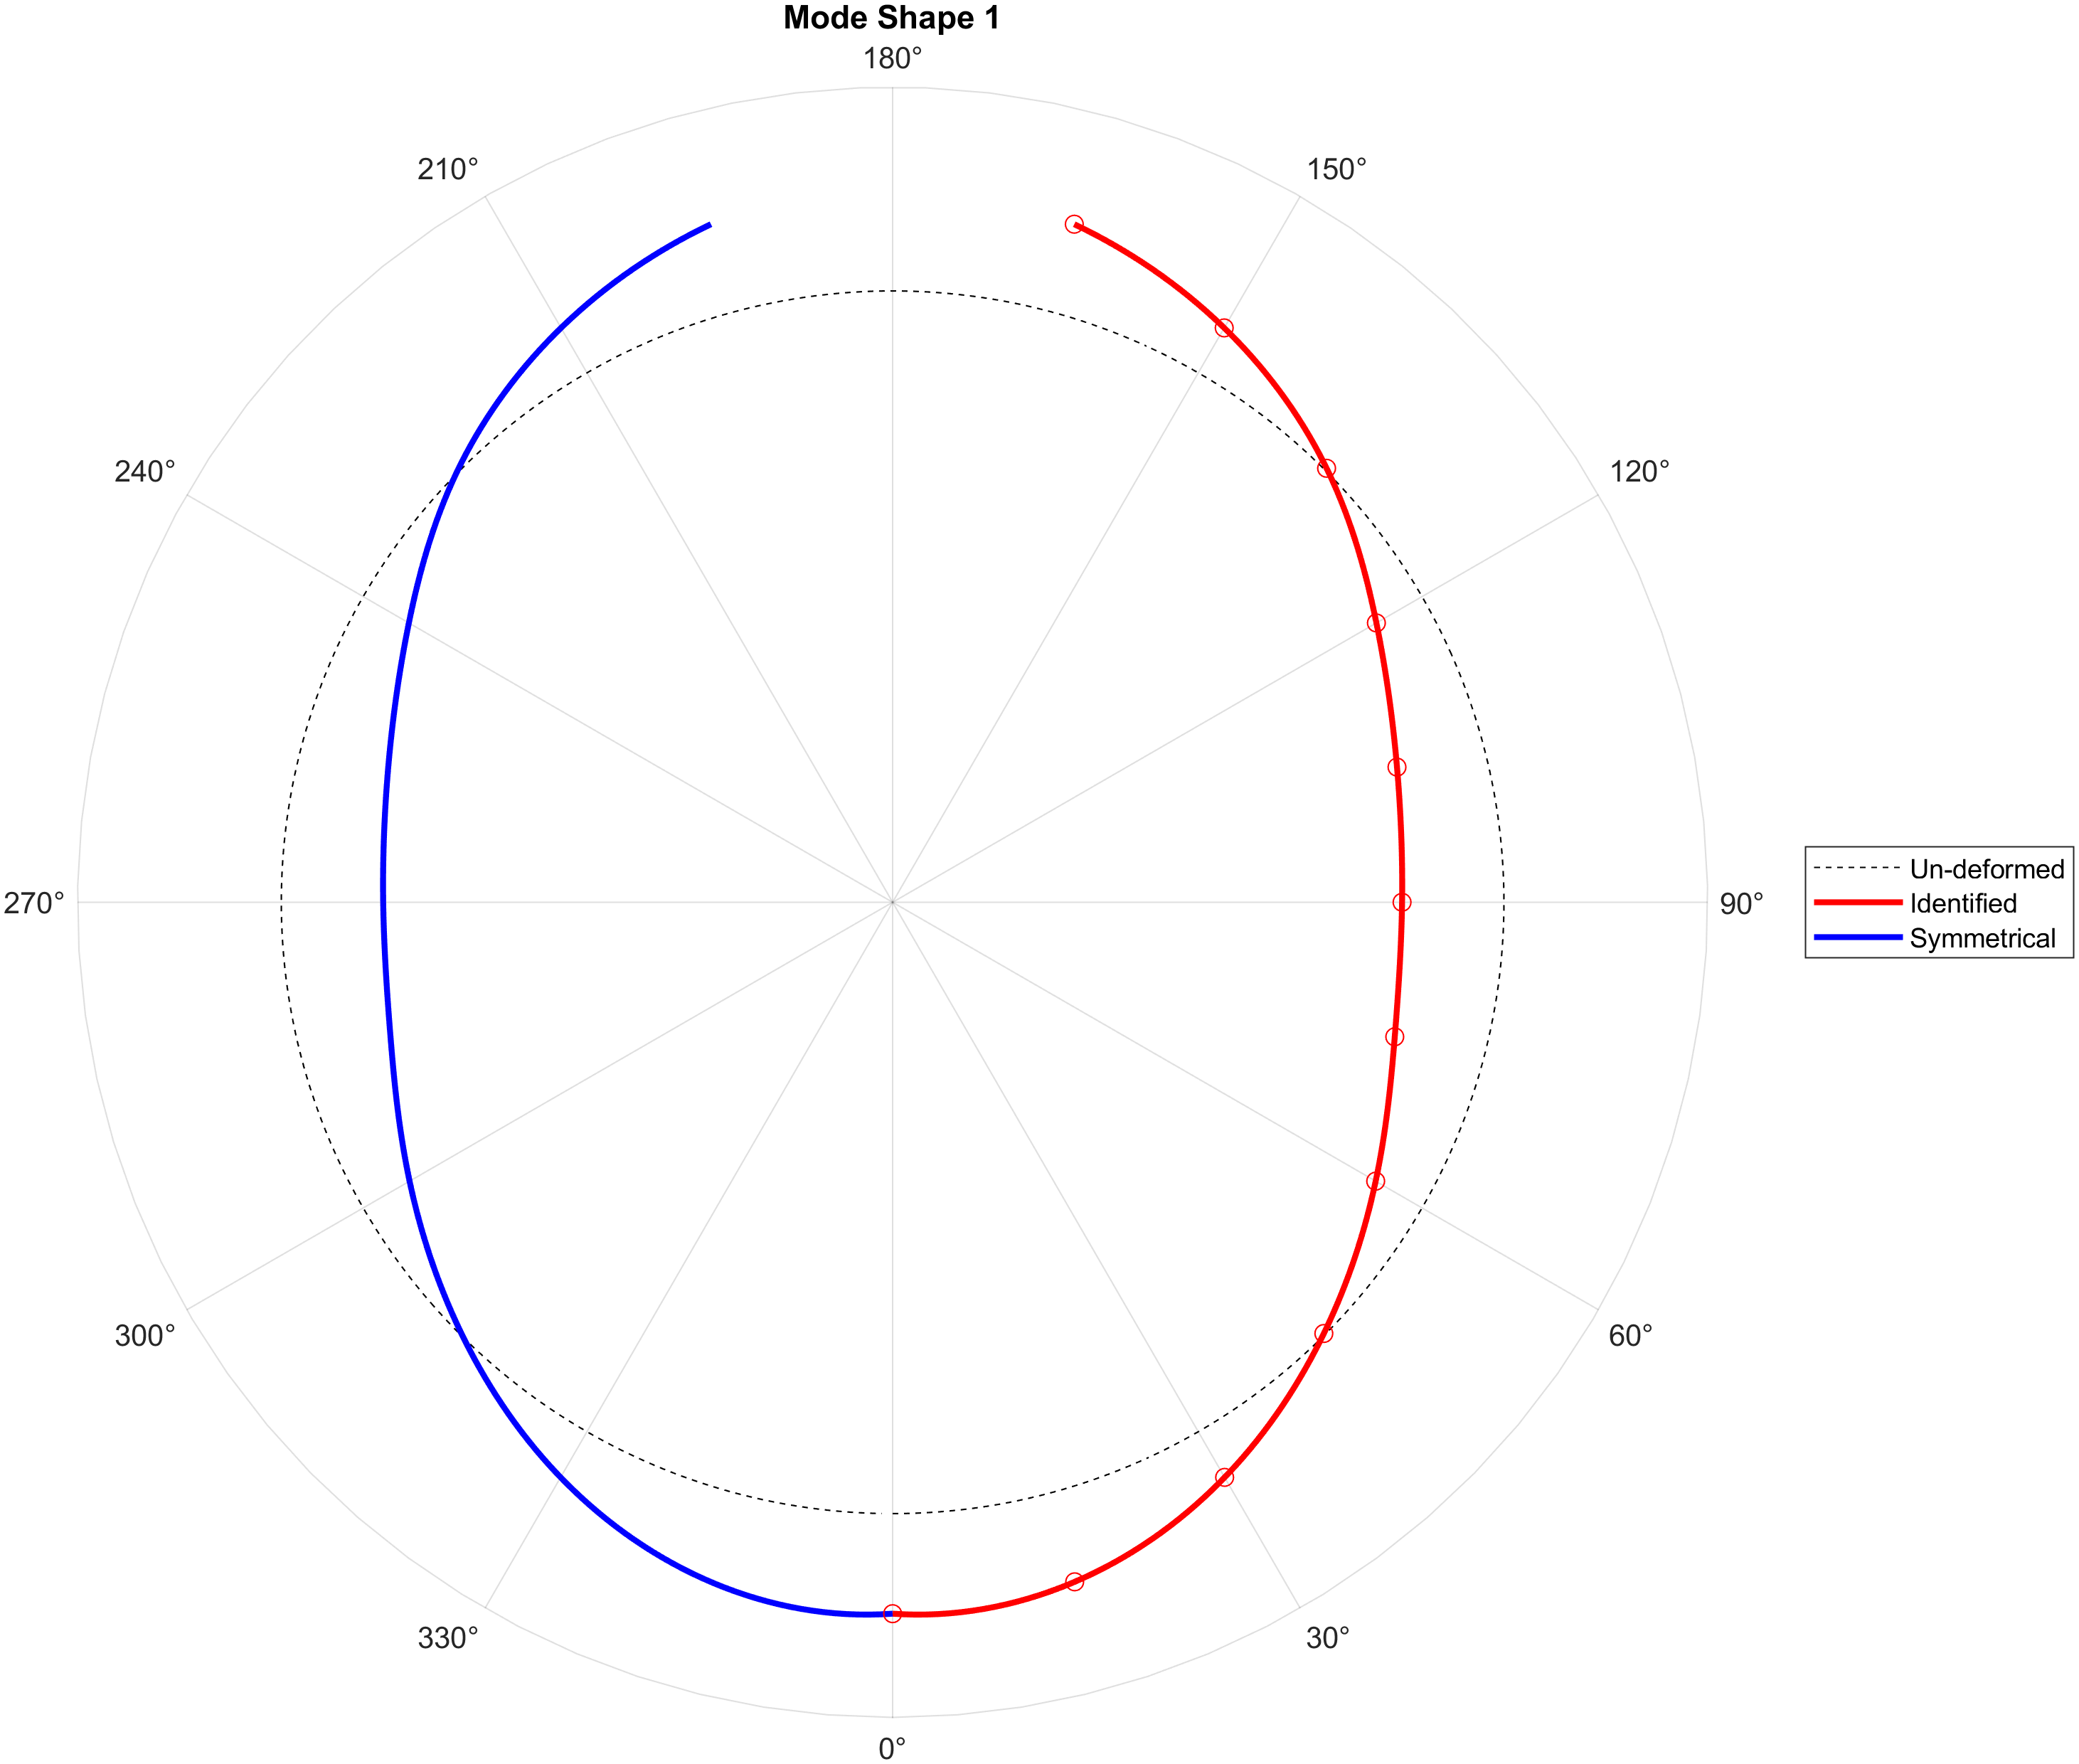
\includegraphics[width=0.45\textwidth]{img/MATLAB/Part_B/ModeShape_01.png}
    \hfill
    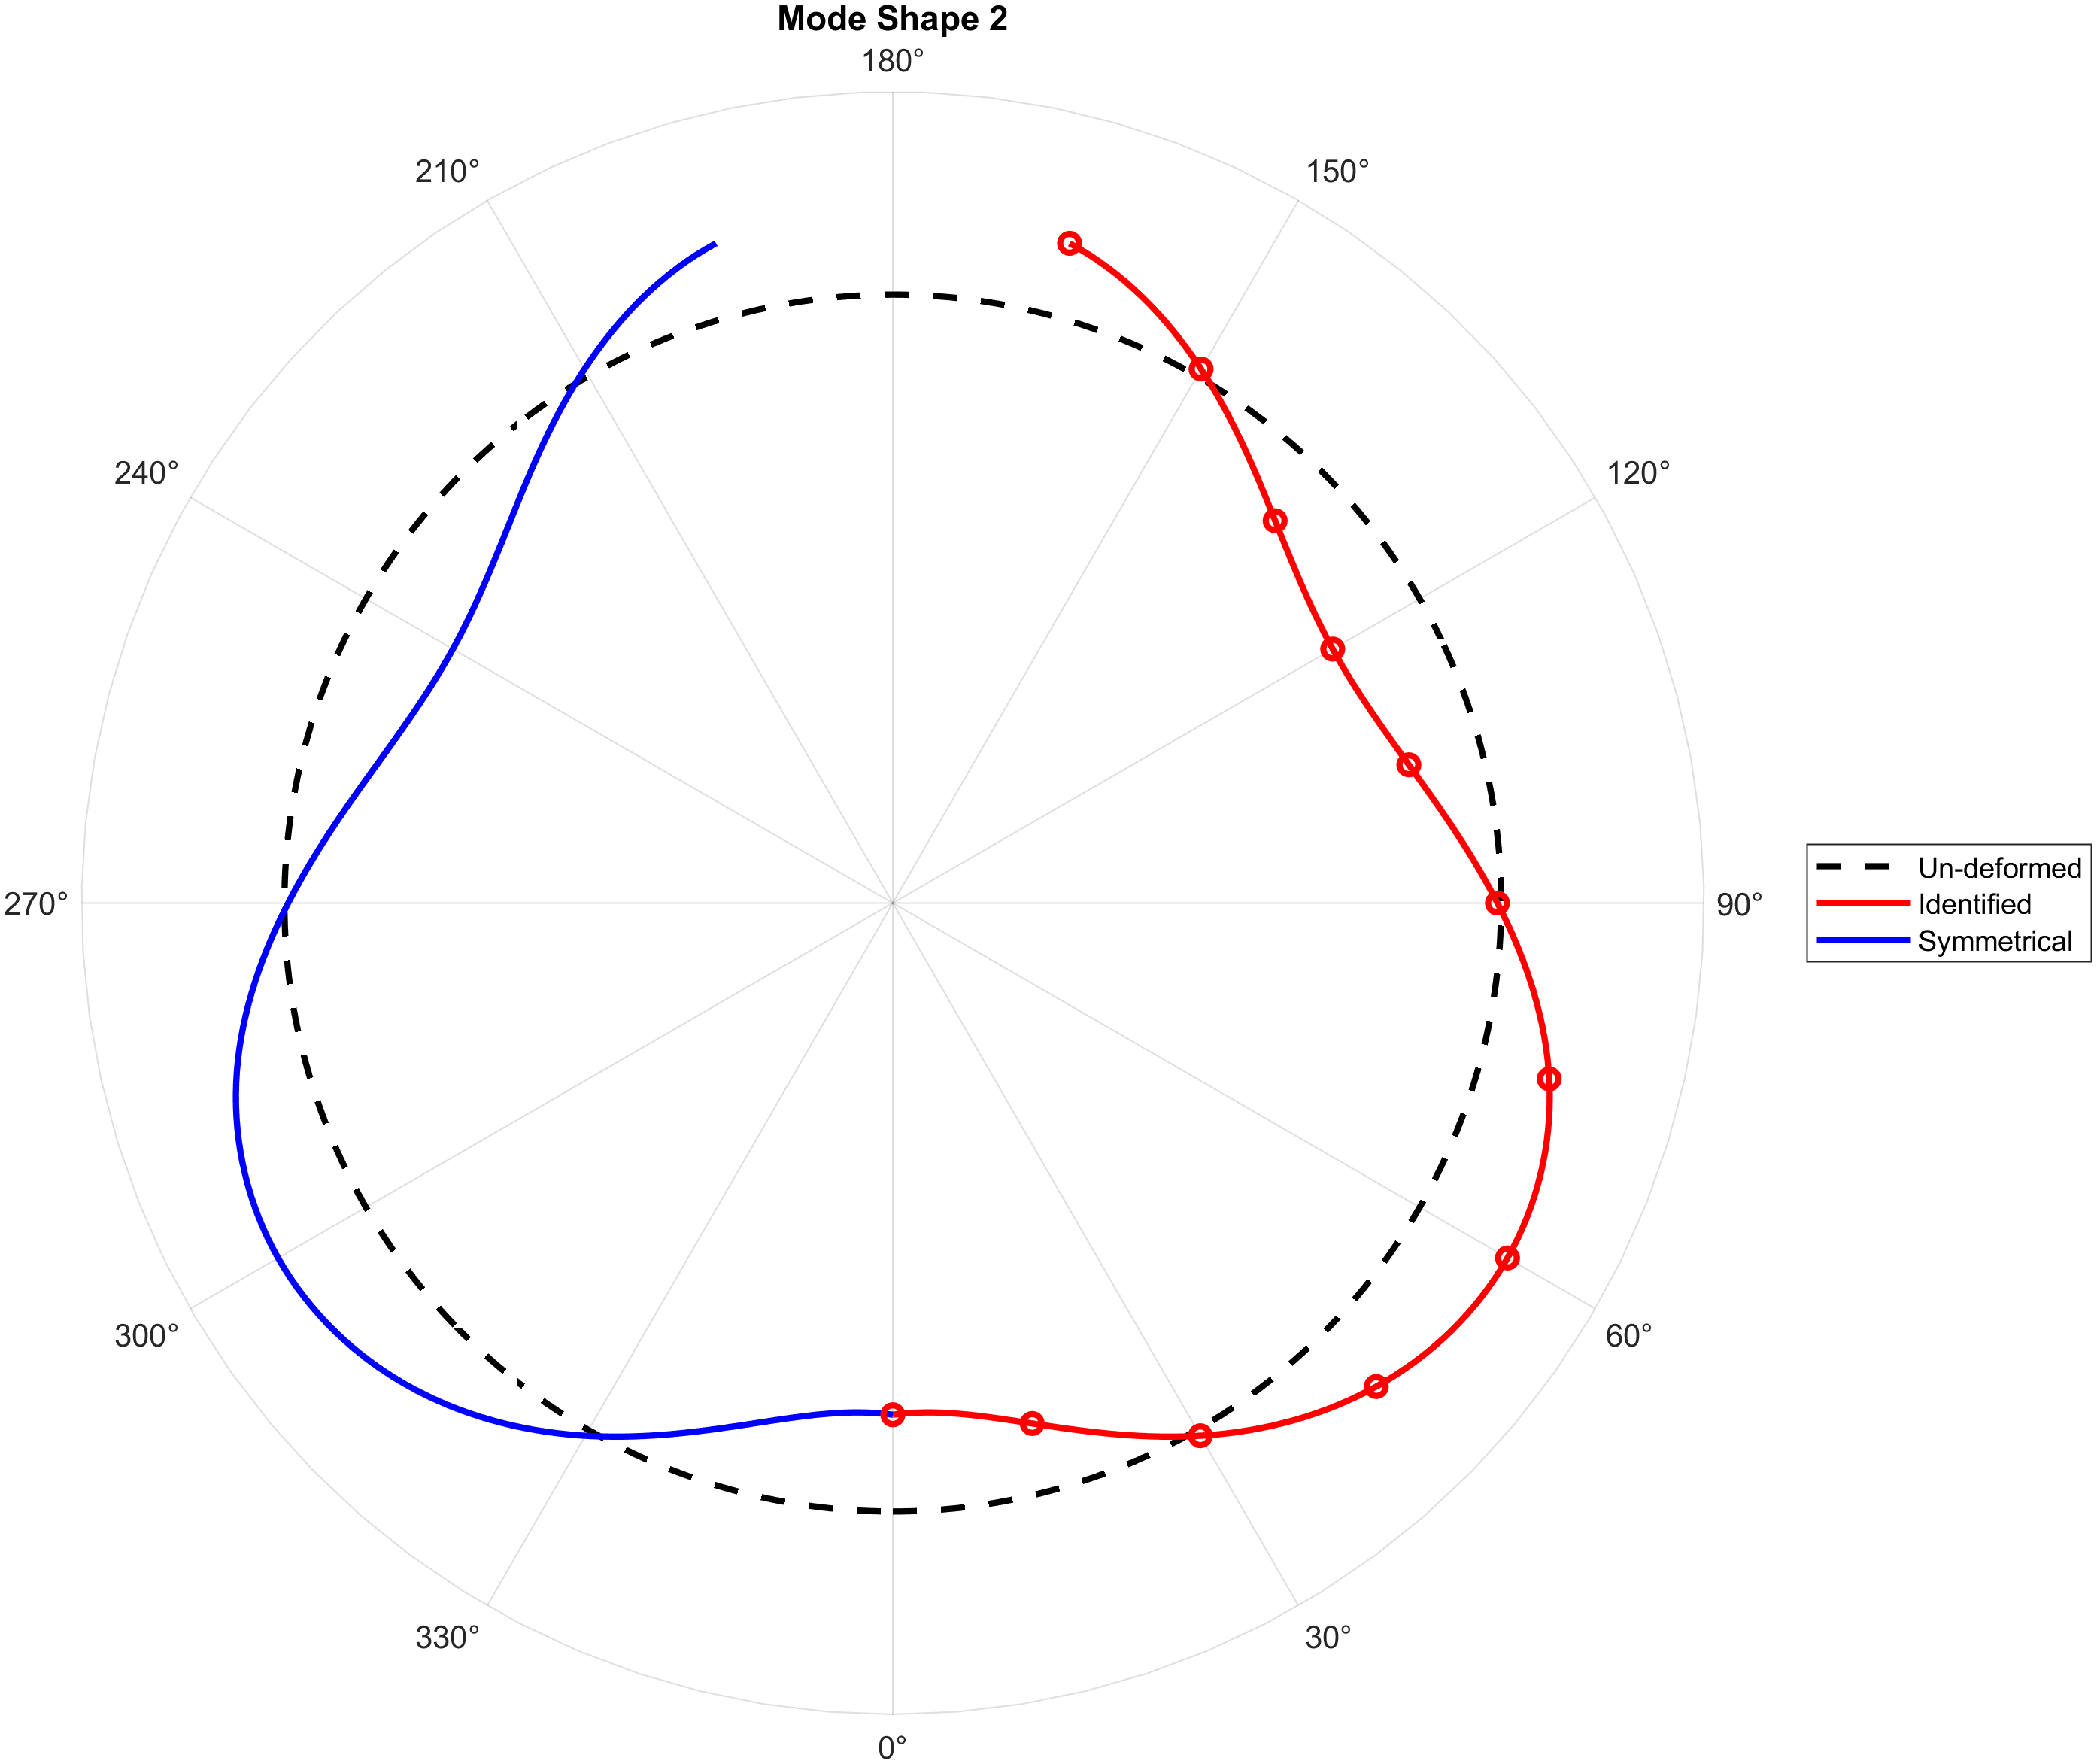
\includegraphics[width=0.45\textwidth]{img/MATLAB/Part_B/ModeShape_02.png}
    \caption{Identified (numerically) first two mode shapes of the system.}
    \label{fig:mode_shapes}
\end{figure}

As a final remark, we report in Table \ref{tab:mode_shapes_parameters} the identified parameters for the first two mode shapes of the system.

\begin{center}
    \huge{Table values to be replaced with the correct ones.}
\end{center}

\begin{table}[H]
    \centering
    \begin{tabular}{lcc}
        \hline
        Mode & Frequency [Hz] & Damping ratio [\%] \\
        \hline
        1    & 0.0            & 0.0                \\
        2    & 0.0            & 0.0                \\
        \hline
    \end{tabular}
    \caption{Identified parameters for the first two mode shapes of the system.}
    \label{tab:mode_shapes_parameters}
\end{table}

